% @file conlusion.tex
% @project IAL Náhradní projekt - 05. Rovinnost grafu
% @author Vladimir Meciar (xmecia00)
% @brief This file is module for documentation.tex with final logic for program
% @changes 7.12.2022
\section{Finální logika}

Na Testování rovinnosti existuje několik podmínek.
Bohužel většina z nich je len postačující, ne nutné.
Jedinné co zůstalo použít je Kuratowského teorém. Jeho řešení spočívá v tom ze sa snažíme v grafu najít podgraf grafu
\ref{fig:graph-k5} a \ref{fig:graph-k33}. Bohužel, nevýhoda tohoto algoritmu je neefektivita. Musime porovnat hodně vrcholů mezi sebou.

\begin{figure}[h]
    \centering
    \begin{subfigure}[b]{0.4\textwidth}
        \centering
        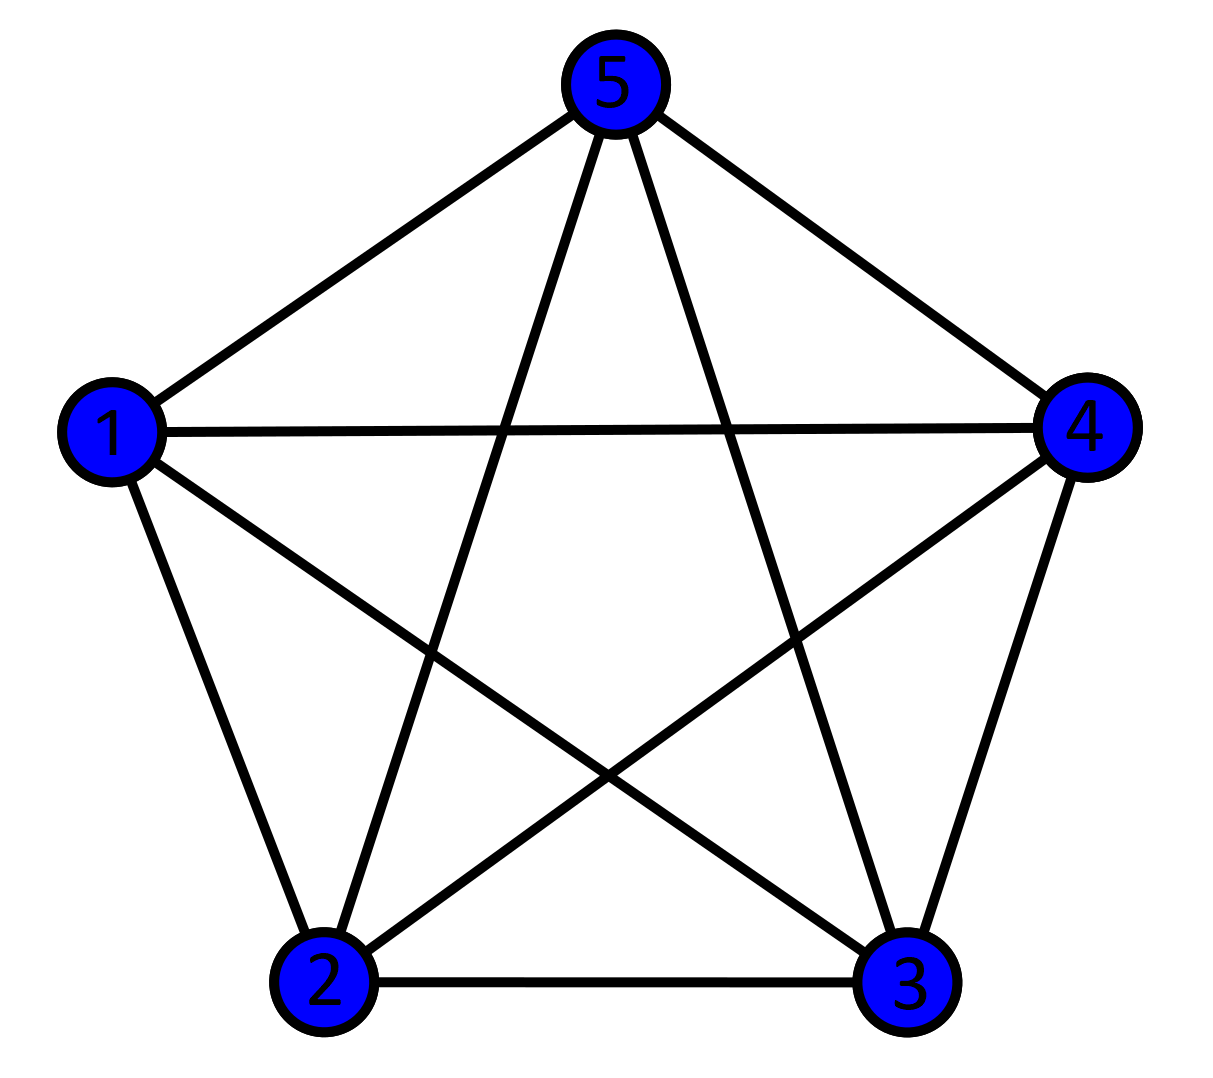
\includegraphics[width=\textwidth]{doc/fig/K5.png}
        \caption{Graf $K_5$}
        \label{fig:graph-k5}
    \end{subfigure}
    \hfill
    \begin{subfigure}[b]{0.3\textwidth}
        \centering
        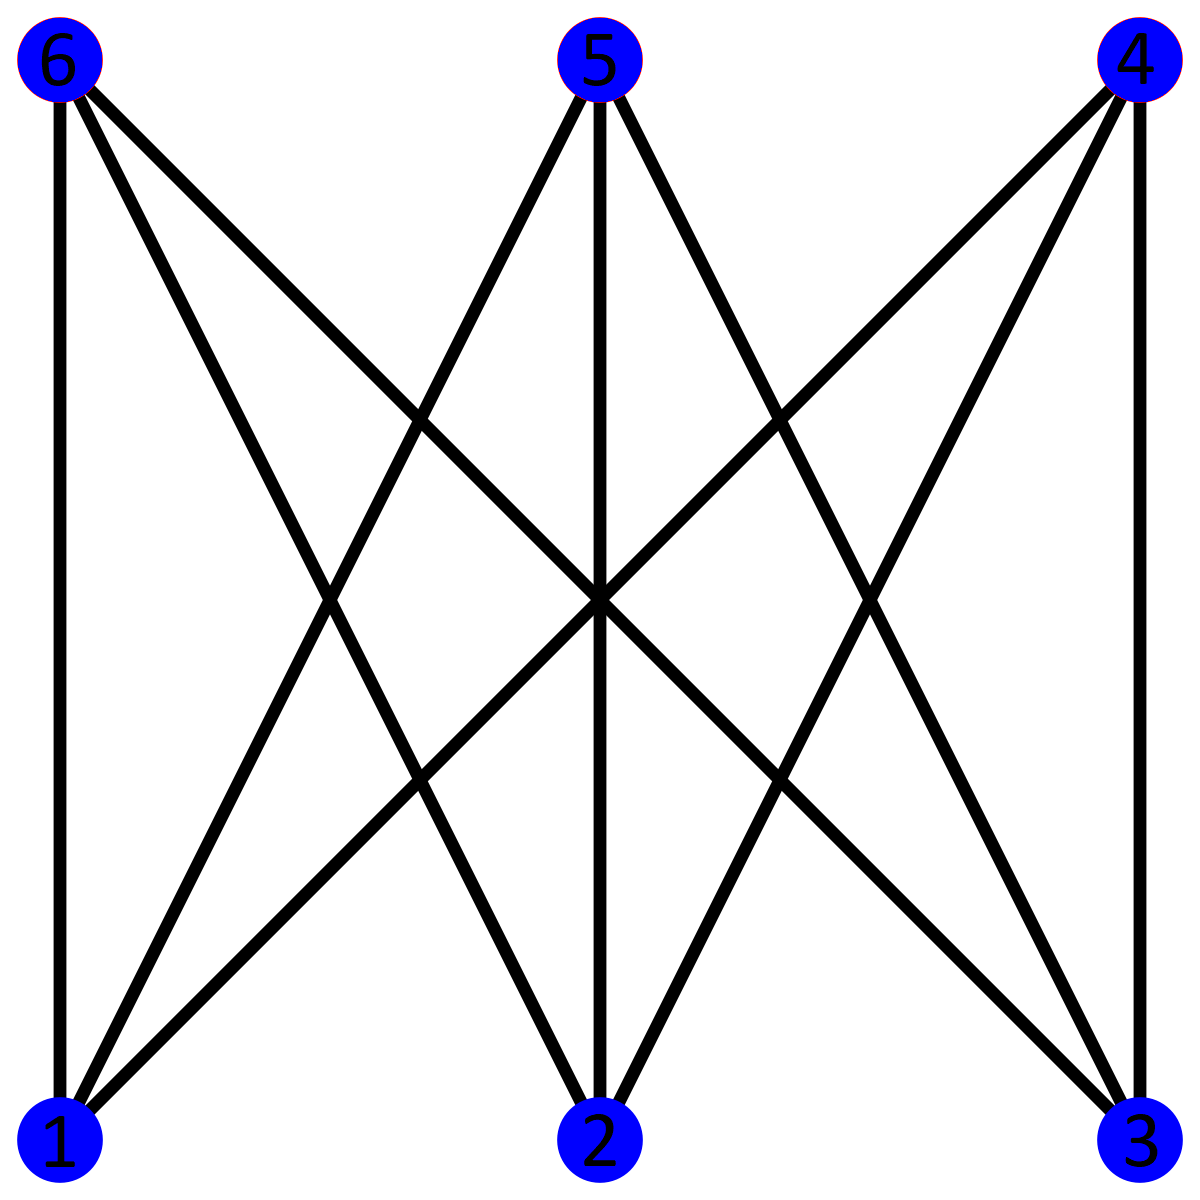
\includegraphics[width=\textwidth]{doc/fig/K33.png}
        \caption{Graf $K_{3,3}$}
        \label{fig:graph-k33}
    \end{subfigure}
    \caption{Nelinearne grafy}
    \label{fig:non_planar_graphs}
\end{figure}
